\begin{center}
    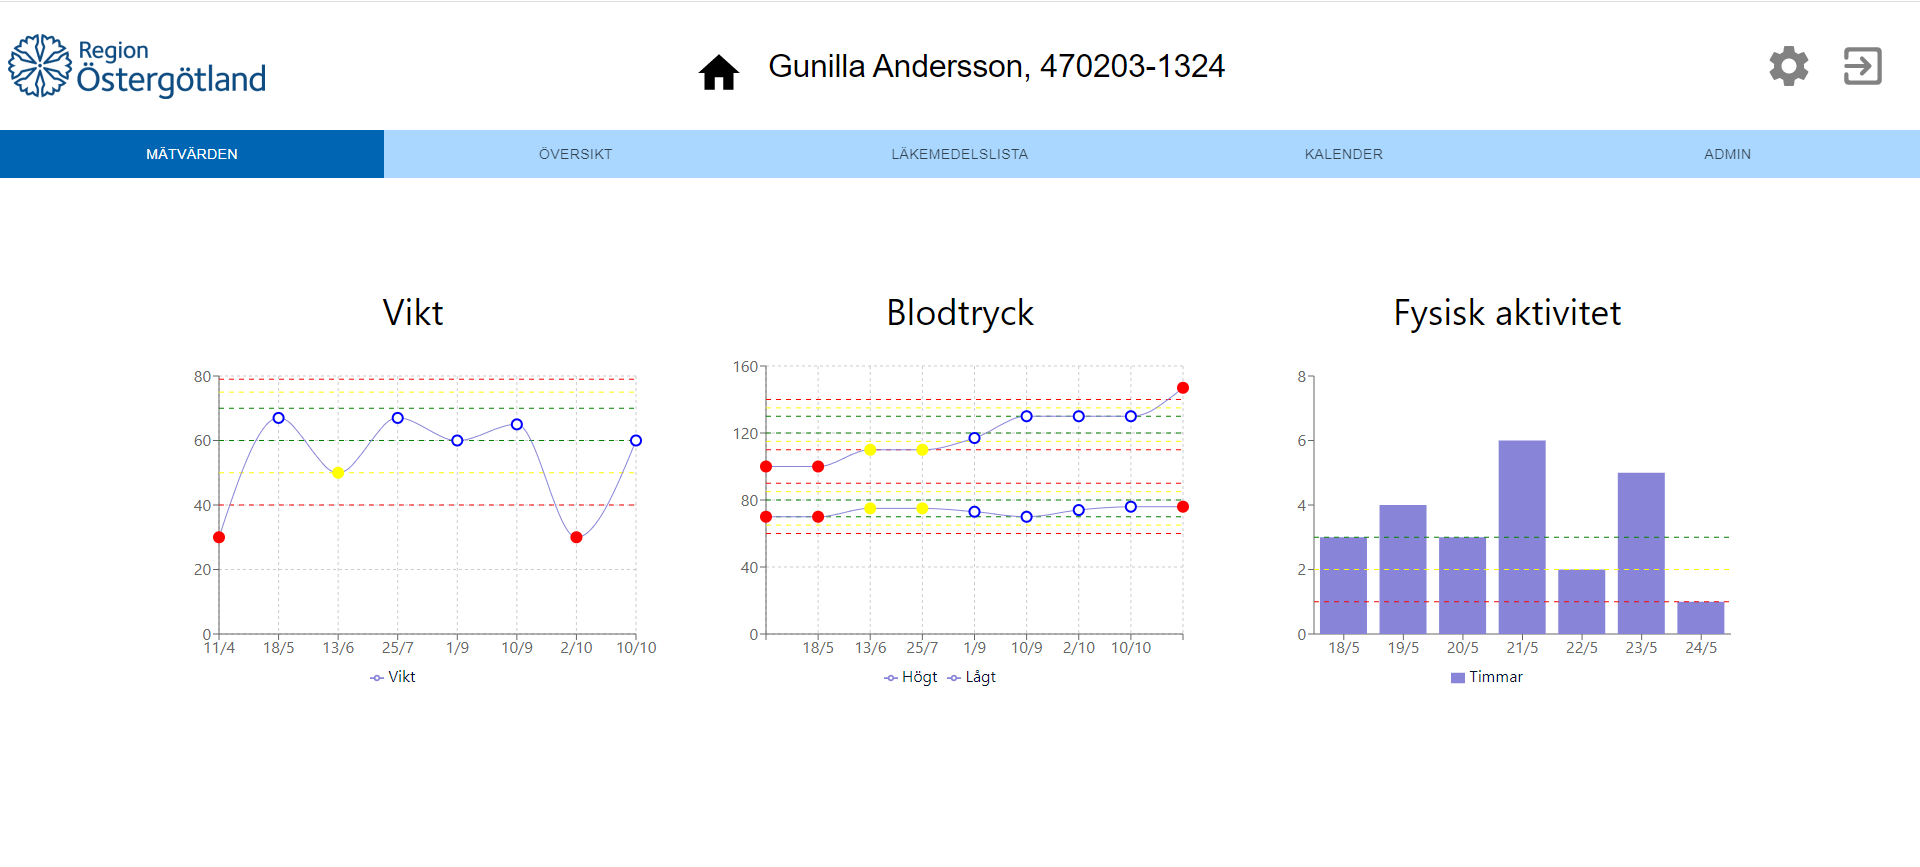
\includegraphics[width=\linewidth]{images/single_patient_measurement_overview_image.png}
    \captionof{figure}{Measurement - overview }
    \label{fig:figures}
\end{center}
All the current measurements for the specific patient are displayed in graphs. In the graph a target range is displayed but also intervals of when a red or yellow warning should be triggered. Measurement points are also seen and if they are outside the allowed references, they become red or yellow depending on severeness. By clicking on a graph you move to the specific measurement were more info and options are displayed
\\

\begin{center}
    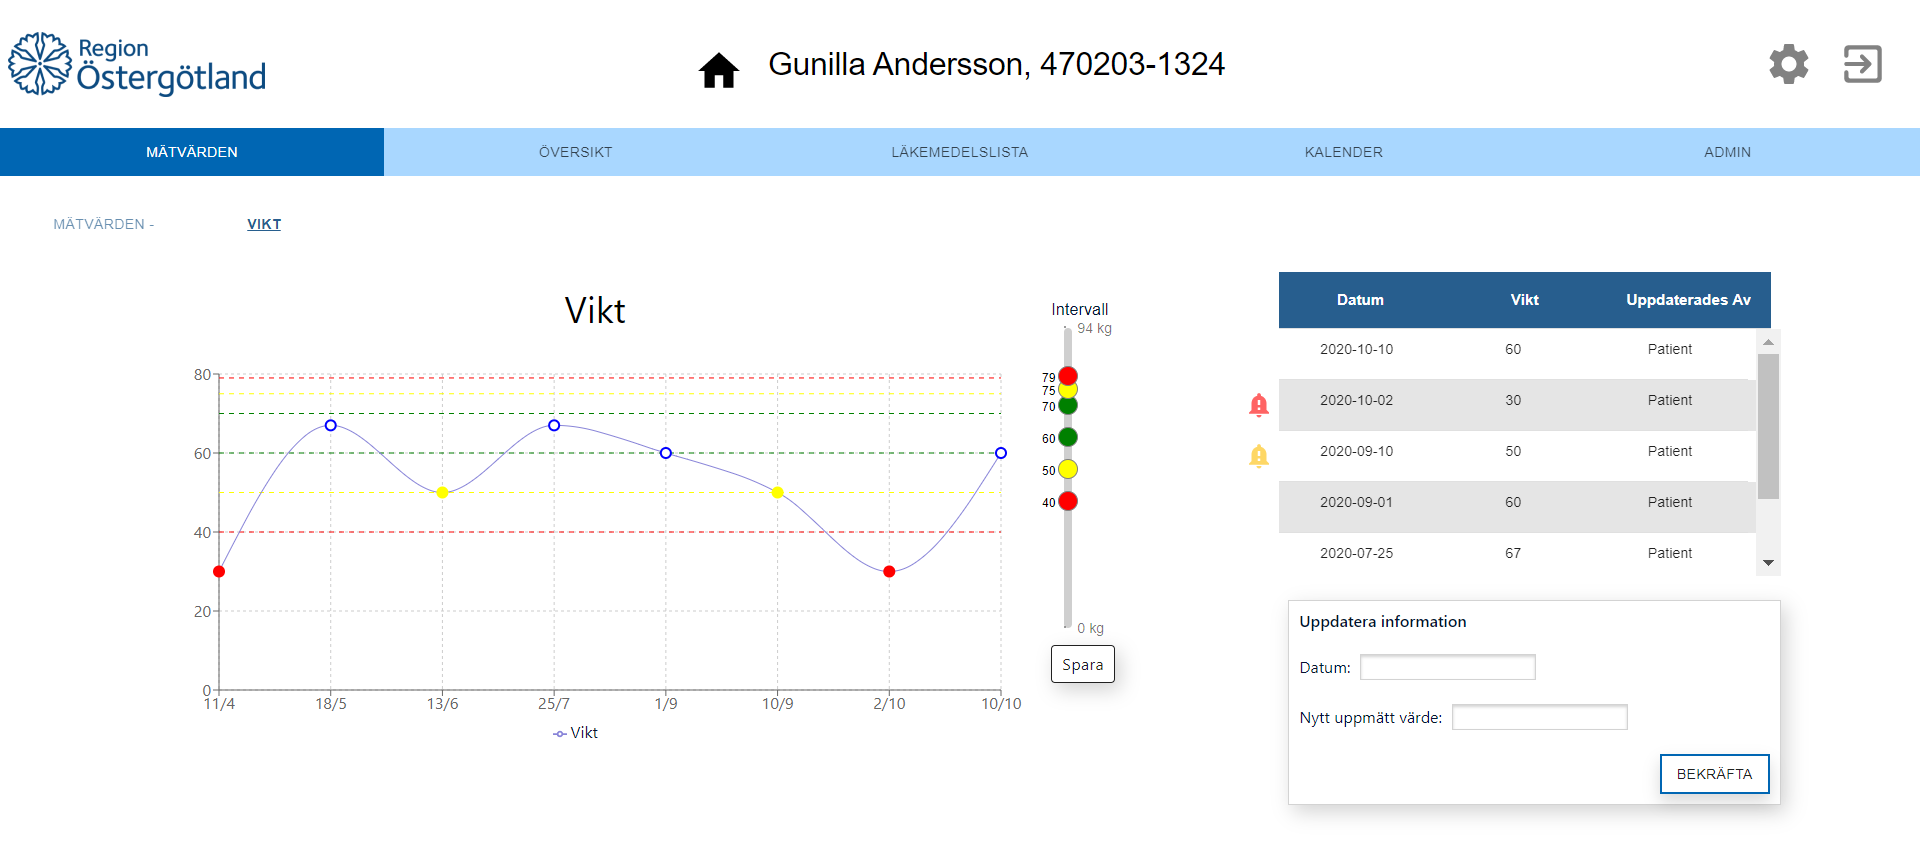
\includegraphics[width=\linewidth]{images/single_patient_weight_measurements_image.png}
    \captionof{figure}{Measurement - single page}
    \label{fig:figures}
\end{center}
On the specific page for a single measurement page, the graph works exactly like before. 

There is also a table at the page were it is possible to click on the notifications for handle the value. When clicking on the notification a pop-up window appears which is described further later. 

----------
\newline
Not fully implemented: 
For admins it is possible to change the reference ranges by moving the green, yellow and red dots displayed to the right of the graph and then click "Spara" (Save). The green dots corresponds to the target value, the yellow to severeness level yellow and the red to severeness level red. 

It is possible to add a new value by filling in the forms "Uppdatera information". Add a date and measure and click on the "Bekräfta" button.
\newline
---------

All the different subpages for specific measurements looks the same, except for that the number of target ranges and reference ranges could vary, for example blood pressure has two, one for systolic pressure and one for dystolic pressure.
\\

\begin{center}
    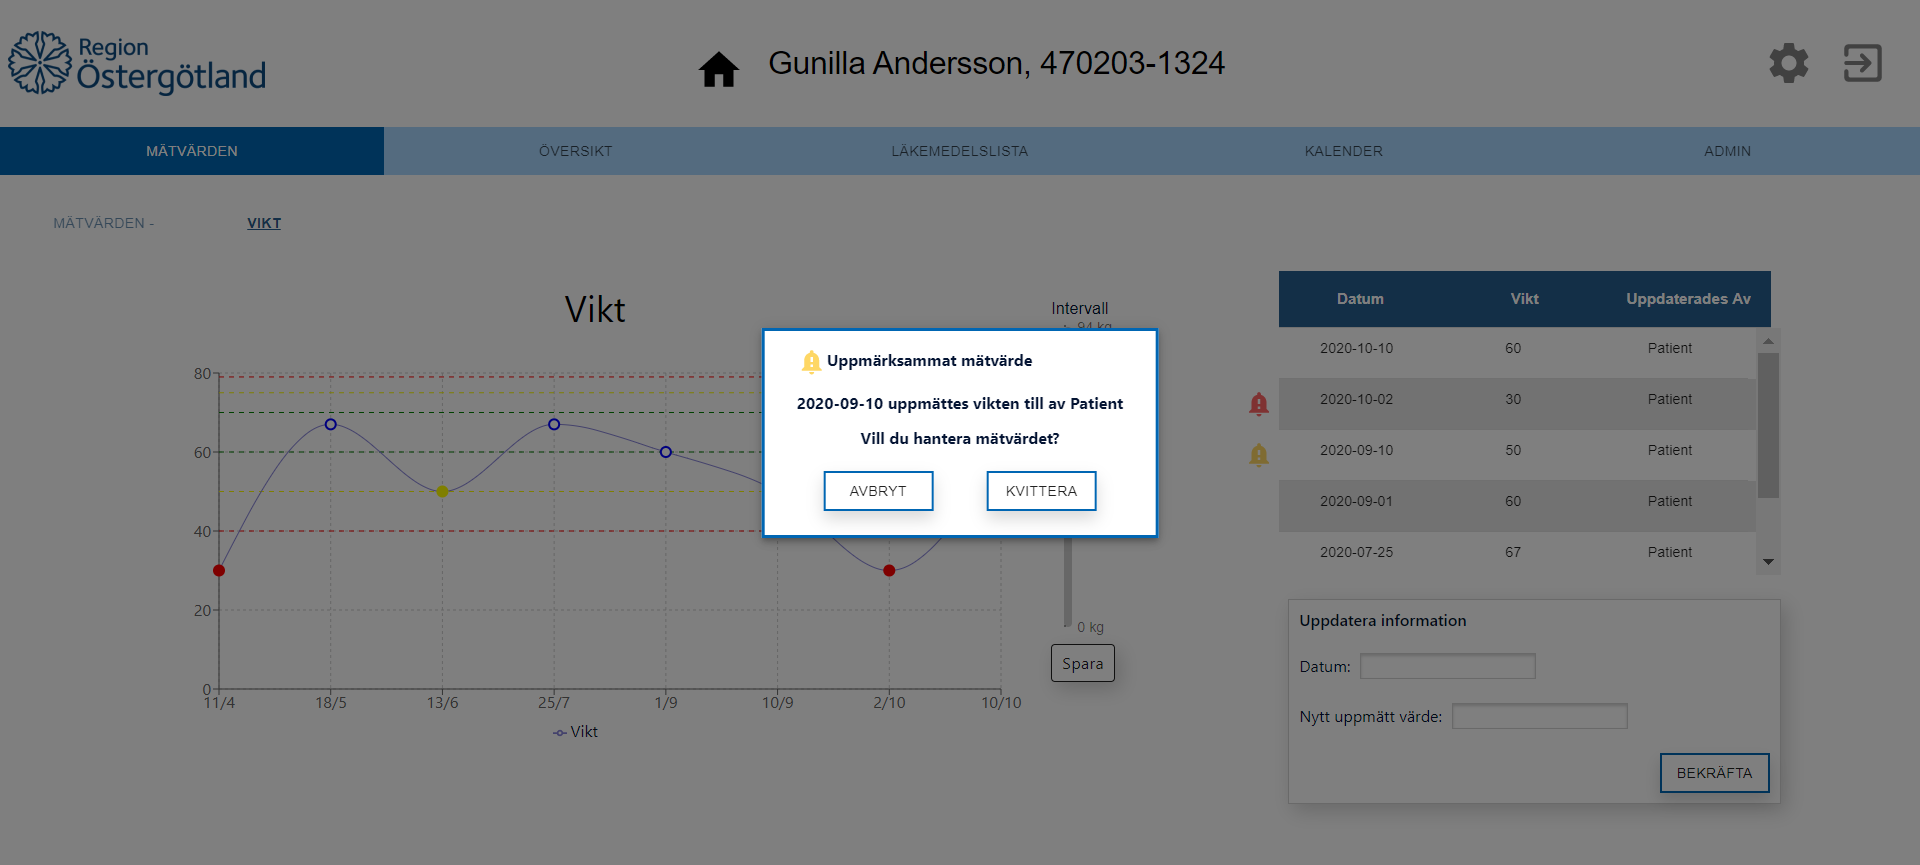
\includegraphics[width=\linewidth]{images/single_patient_weight_measurements_handle1_image.png}
    \captionof{figure}{Measurement - handle change 1 }
    \label{fig:figures}
\end{center}
When clicking on a notification a pop-up window appears with two options, "Avbryt" and "Kvittera". By clicking on "Avbryt" the pop-up window shuts down and nothing happen. By clicking on "Kvittera" another pop-up appears which is described below.
\\

\begin{center}
    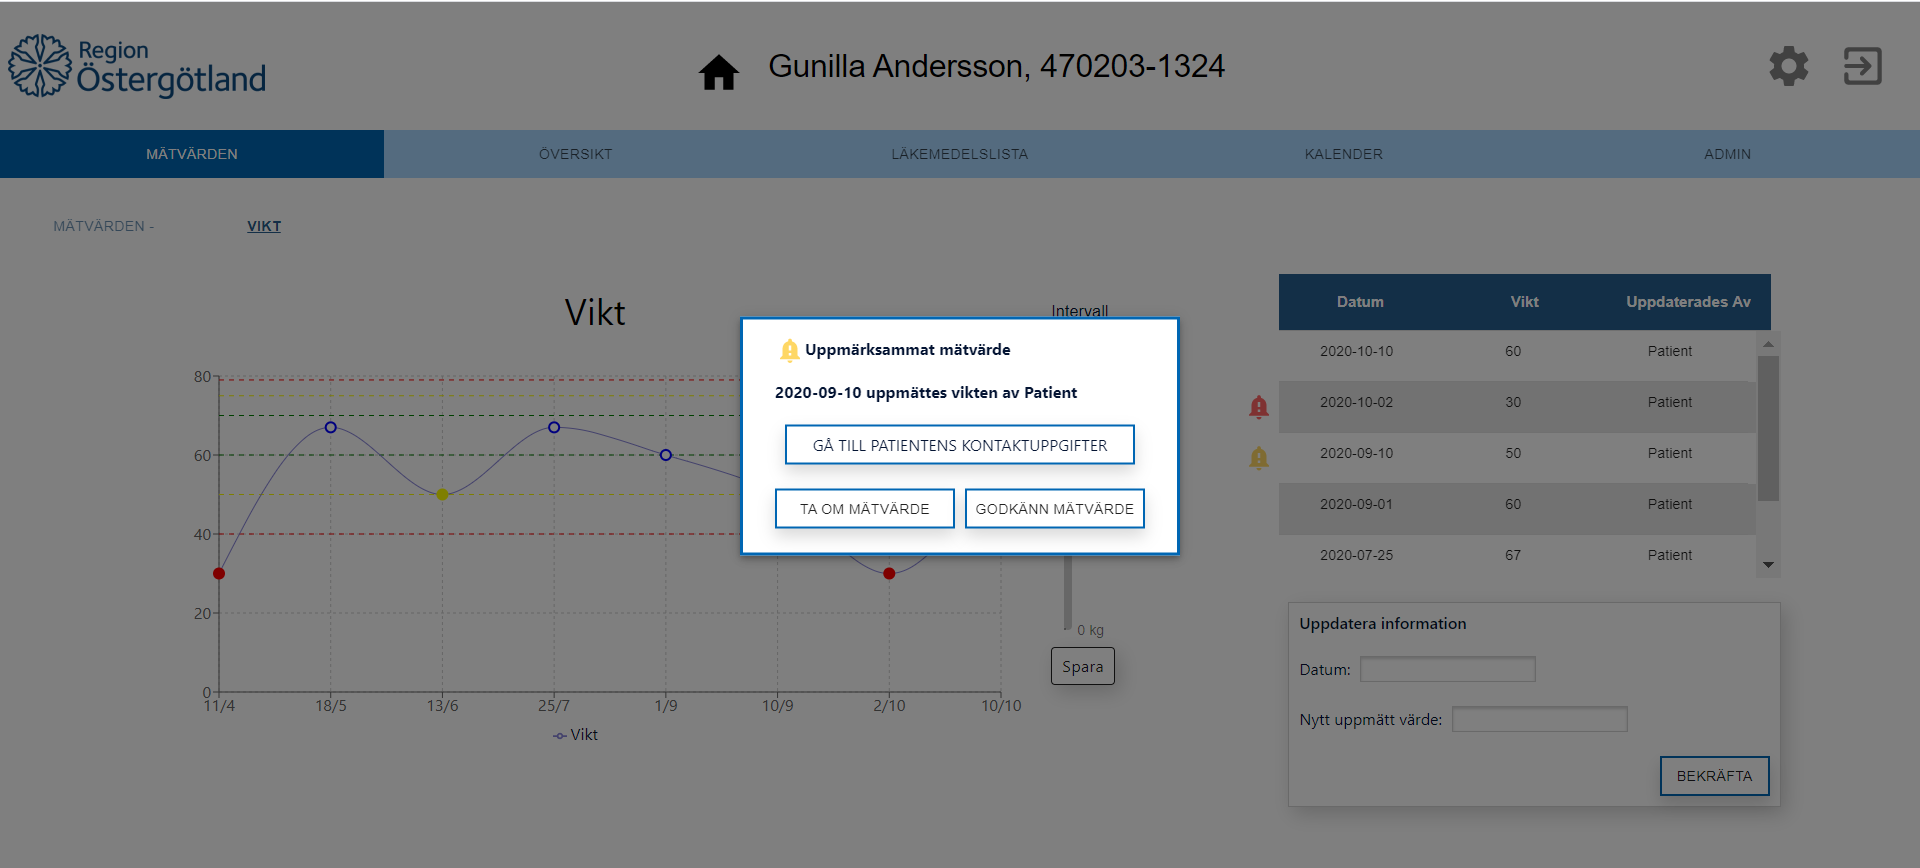
\includegraphics[width=\linewidth]{images/single_patient_weight_measurements_handle2_image.png}
    \captionof{figure}{Measurement - handle change 2 }
    \label{fig:figures}
\end{center}
If clicked on the "Kvittera" button there is now three alternatives. By clicking on "Gå till patientens kontaktuppgifter" you are moved to "patient/overview". By clicking on "Ta om mätvärde" a request is sent to the patient to retake the measured value. By clicking on "Acceptera mätvärde" the notification is taken away.
\\